\section{Dynamics:  Motion in a Plane}

\subsection{Uniform Circular Motion}

\begin{definition}[Uniform Circular Motion]
    Something that moves in a circle at constant speed, the magnitude of
    the velocity.
\end{definition}

Figure~%
\ref{fig:uniform-circular-motion} shows a particle moving around a
circle of radius
$
    r
$%
.
\begin{remark}
    While the magnitude of velocity never changes, the velocity is not
    constant as the direction of the velocity changes.
\end{remark}
\begin{figure}
    \centering
    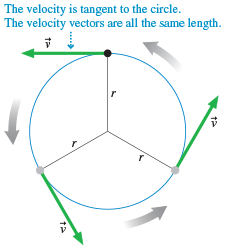
\includegraphics[width=0.6\textwidth]{../figures/uniform-circular-motion.png}
    \caption{A particle in uniform circular motion.}%
    \label{fig:uniform-circular-motion}
\end{figure}

\begin{definition}[Revolution]
    The time interval it takes an object to go around a circle once.
    The period of the motion.  Represented by symbol
    $
        T
    $%
    .
\end{definition}

In one period, the particle moves around a circle of radius
$
    r
$%
, thus
\begin{equation}
    \label{eq:avg-circular-speed} v_{t}=\frac{2\pi r}{T}
\end{equation}

\subsection{Angular Position}

Rather than using a cartesian plane, it will be more convient to
describe the position of a particle in circular motion by its distance
$
    r
$ from the center of the circle and its angle
$
    \theta
$ from the positive x-axis.  This is shown in Figure~%
\ref{fig:angular-position}
\begin{figure}
    \centering
    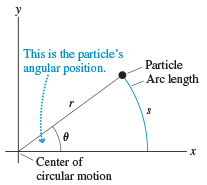
\includegraphics[width=0.6\textwidth]{../figures/angular-position.png}
    \caption{A particle's position is described by distance
    $
        r
    $ and angle
    $
        \theta
    $%
    .}%
    \label{fig:angular-position}
\end{figure}

While degrees are used to measure angle, it can be more useful to
measure the angle
$
    \theta
$ in Figure~%
\ref{fig:angular-position} by using the \textbf{arc length}
$
    s
$ that the particle travels along the edge of a circle of radius
$
    r
$%
.  We define the angular unit of \textbf{radians} such that
\begin{equation}
    \label{eq:radian-def} \theta \coloneqq \frac{s}{r}
\end{equation}
The radian is the SI unit of angle.

The arc length completely around a circle is the circle's circumference.
Thus the angle of a full circle is

\begin{equation}
    \theta_{\mathrm{full~circle}}=\frac{2\pi r}{r}=\SI{2\pi}{\radian}
\end{equation}

The motivation behind using radians is there is an important consequence
behind Equation~%
\ref{eq:radian-def}
\begin{equation}
    \label{eq:radian-motivation} s=r\theta
\end{equation}

\subsection{Angular Velocity}

\begin{definition}[Angular Velocity]
    The rate of change
    $
        \theta
    $ over time.
\end{definition}

\begin{figure}
    \centering
    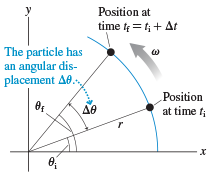
\includegraphics[width=0.6\textwidth]{../figures/angular-velocity.png}
    \caption{A particle moves with angular velocity
    $
        \omega
    $%
    .}%
    \label{fig:angular-velocity}
\end{figure}

Figure~%
\ref{fig:angular-velocity} shows a particle moving in a circle from an
initial angular position
$
    \theta_i
$ at time
$
    t_i
$ to a final angular position
$
    \theta_f
$ at a later time
$
    t_f
$%
.  We can measure the particle's circular motion in terms of the rate of
change of
$
    \theta
$%
.
\begin{equation}
    \mathrm{average angular velocity} \coloneqq \frac{\Delta\theta}{\Delta
    t}
\end{equation}
We can find the \textbf{instantaneous angular velocity} by
\begin{equation}
    \omega \coloneqq \lim_{\Delta t\to 0} \frac{\Delta\theta}{\Delta t}
    = \frac{d\theta}{dt}
\end{equation}
\begin{remark}
    A particle moves with uniform circular motion if and only if its
    angular velocity
    $
        \omega
    $ is constant and unchanging
\end{remark}

As a particle goes around a circle one time, its angular displacement is
$
    \Delta\theta=\qty{2\pi}{\radian}
$ during the interval
$
    \Delta t = T
$%
.  Thus, we can find the average angular velocity by
\begin{equation}
    \label{eq:avg-angular-velocity} |\omega_{\mathrm{average}}|=\frac{\qty
    {2\pi}{\radian}}{T}
\end{equation}

Combining Equation~%
\ref{eq:avg-angular-velocity} and Equation~%
\ref{eq:avg-circular-speed}, we see that the tangential velocity and the
angular velocity are related by
\begin{equation}
    \label{eq:tangential-angular-velocity-relationship} v_t=\omega r
\end{equation}

\subsection{Centripetal Acceleration}

\begin{figure}
    \centering
    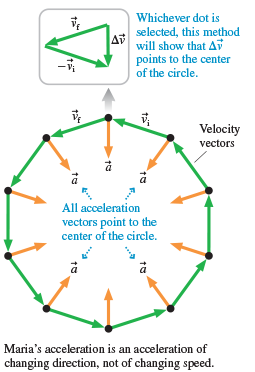
\includegraphics[width=0.6\textwidth]{../figures/centripetal-acceleration.png}
    \caption{Constant speed, but not velocity.}%
    \label{fig:celtripetal-acceleration}
\end{figure}

Figure~%
\ref{fig:circular-motion-acceleration} shows a motion diagram of Maria
riding a ferris wheel.  She has constant speed, but not velocity because
the direction is changing.  She may not be speeding but, but she is
accelerating.

\begin{definition}[Centripetal Acceleration]
    Acceleration that points inward, "center seeking."
\end{definition}

\begin{figure}
    \centering
    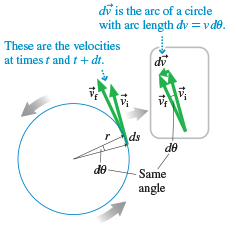
\includegraphics[width=0.6\textwidth]{../figures/finding-circular-motion-acceleration.png}
    \caption{Finding the acceleration of circular motion.}%
    \label{fig:circular-motion-acceleration}
\end{figure}

We can prove that the acceleration of uniform circular motion is
centripetal by finding a value for
$
    \vec{a}
$%
.  Figure~%
\ref{fig:circular-motion-acceleration} shows the velocity
$
    \vec{v}_i
$ at one instant of motion and the velocity
$
    \vec{v}_f
$ an infinitesimal amount of time
$
    dt
$ later.  During this small interval of time, the particle has moved
through the infinitesimal angle
$
    d\theta
$ and traveled an infinitesimal distance
$
    ds=r{d\theta}
$%
.  By definition, the acceleration is
\begin{equation}
    \vec{a}=\frac{d\vec{v}}{dt}
\end{equation}
Since
$
    dt
$ is a scalar, it is only scaling
$
    d\vec{v}
$%
.  Because
$
    d\vec{v}
$ is pointing to the inside of the circular, the acceleration will too.

The magnitude of
$
    \vec{a}
$ is
$
    \frac{v^2}{r}
$%
.  Using Equation~%
\ref{eq:tangential-angular-velocity-relationship}, we can also express
the magnitude of centripetal acceleration in terms of the angular
velocity
$
    \omega
$ as
\begin{equation}
    \vec{a}=\left(\omega^2r,\mathrm{toward~center~of~circle}\right)
\end{equation}

\subsection{Uniform Circular Motion rtz}

\begin{figure}
    \centering
    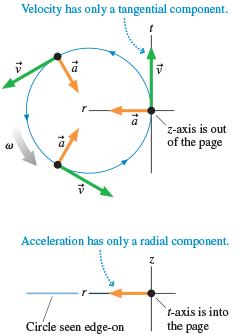
\includegraphics[width=0.4\textwidth]{../figures/rtz-coordinates.png}
    \caption{Uniform circular motion and the \emph{rtz}-coordinate
    system.}%
    \label{fig:rtz-coordinates}
\end{figure}

An \emph{xy}-coordinate system is not a good choice to analyze circular
motion because the
$
    x
$- and
$
    y
$- components of the acceleration are not constant.  Instead, as Figure~%
\ref{fig:rtz-coordinates} shows, we'll use a relative coordinate system
whose axes are defined as follows:
\begin{enumerate}
    \item
        The origin is the point where the particle is located.
    \item
        The
        $
            r
        $-axis (radial-axis) points \emph{from} the particle \emph{toward}
        the center of the circle
    \item
        The
        $
            t
        $-axis (tangent axis) is tangent to the circle, pointing in the
        ccw direction.
    \item
        The
        $
            z
        $-axis is perpendicular to the plane of motion.
\end{enumerate}

Now we can address each point on Figure~%
\ref{fig:rtz-coordinates} with the
$
    rtz
$-components of
$
    \vec{v}
$ and
$
    \vec{a}
$%
.
\noindent
\begin{minipage}{.5\linewidth}
    \begin{align*}
        v_r &= 0 \\
        v_t &= \omega r \\
        v_z &= 0
    \end{align*}
\end{minipage}
\begin{minipage}{.5\linewidth}
    \begin{align*}
        a_r &= \frac{v^2}{r} = \omega^2r \\
        a_t &= 0 \\
        a_z &= 0
    \end{align*}
\end{minipage}

\subsection{Dynamics of Uniform Circular Motion}

For a particle in uniform circular motion, Newton's Second Law tells us
how much net force is needed to cause the acceleration:
\begin{equation}
    \fnet = m\vec{a} = \left(\frac{mv^2}{r},\mathrm{towards~center~of~circle}\right)
\end{equation}

\begin{Exercise}[title={Spinning in a Circle}, origin={Knight}]
    A father places his \SI{20}{\kilogram} child on a \SI{5.0}{\kilogram}
    cart to which a \SI{2.0}{\metre} long rope is attached.  He spins
    the cart around in a circle by the rope parallel to the ground at a
    constant tension of \SI{100}{\newton}, how many rpm does the cart
    make?
\end{Exercise}
\begin{Answer}
    \begin{center}
        \includegraphics[totalheight=0.2\textheight]{../figures/cart-Spinning-model.png}
        \captionof{figure}{Pictorial representation of a cart spinning
        in a circle.}%
        \label{ex:cart-spinning}
    \end{center}

    Using Newton's second law,
    \begin{align}
        \sum F_r &= T = \frac{mv^2}{r} \\
        \sum F_z &= n - mg = 0
    \end{align}
    From the
    $
        F_r
    $ equation we derive an equation for
    $
        v_t
    $ and solve for
    $
        v_t
    $%
    :
    \begin{equation}
        v=\sqrt{\frac{rT}{m}}=\sqrt{\frac{\qty{2.0}{\metre}\qty{100}{\newton}}
        {\qty{25}{\kilogram}}}=\qty{2.83}{\metre\per\second}
    \end{equation}
    The cart's angular velocity is then found from Equation~%
    \ref{eq:tangential-angular-velocity-relationship}:
    \begin{equation}
        \omega=\frac{v_t}{r}=\frac{v}{r}=\frac{\qty{2.83}{\metre\per\second}}
        {\qty{2.0}{\metre}}=\qty{1.41}{\radian\per\second}
    \end{equation}
    Now we convert
    $
        \omega
    $ to rpm:
    \begin{equation}
        \omega=\qty{1.41}{\radian\per\second} \div \qty{2\pi}{\radian}
        \times \qty{60}{\second} = \qty{14}{\revolution\per\minute}
    \end{equation}

\end{Answer}
